\documentclass[11pt]{article}

% Basic packages
\usepackage{amsmath}
\usepackage{graphicx}
\usepackage{parskip}
\usepackage[section]{placeins}
\usepackage[capitalise, noabbrev]{cleveref}
\usepackage{csvsimple}
\usepackage{booktabs}
\usepackage[margin=3cm]{geometry}
\usepackage[table,xcdraw]{xcolor}
\usepackage{tikz}
\usetikzlibrary{math,calc,positioning}

\usepackage[backend=biber]{biblatex}
\bibliography{bibliography}

\usepackage{todonotes}

% Set up fonts
\usepackage{fontspec}
\usepackage{unicode-math}
\setmainfont{STIX Two Text}
\setmathfont{STIX Two Math}

\title{FYS-STK4155 - Project1}
\author{Gard, Are, David Andreas Bordvik}
\date{\today}

\begin{document}

\maketitle
\section*{Theory}
MSE value between $\boldsymbol{y}$ and $\boldsymbol{\hat y}$ is defined as;
\begin{equation}
    MSE(\boldsymbol{y},\boldsymbol{\tilde{y}}) = \frac{1}{n}
    \sum_{i=0}^{n-1}(y_i-\tilde{y}_i)^2
\end{equation}

The $R^2$ value between $\boldsymbol{y}$ and $\boldsymbol{\hat y}$ is defined as;
\begin{equation}
    R^2(\boldsymbol{y}, \tilde{\boldsymbol{y}}) = 1 - \frac{\sum_{i=0}^{n - 1} (y_i - \tilde{y}_i)^2}{\sum_{i=0}^{n - 1} (y_i - \bar{y})^2}
\end{equation}

The mean value of $\boldsymbol{y}$ is defined as;
\begin{equation}
    \bar{y} =  \frac{1}{n} \sum_{i=0}^{n - 1} y_i
\end{equation}

The variance of $\boldsymbol{y}$ is defined as;
\begin{equation}
    \mathrm{var}[\boldsymbol{x}]=\frac{1}{n}\sum_{i=0}^{n-1}(x_i- \overline{x})^2
\end{equation}



\section*{Exercise 1}
\begin{figure}
  \centering
  \includegraphics{figures/franke_function_preview.pdf}
  \caption{?}
  \label{fig: ?}
\end{figure}

\begin{figure}
  \centering
  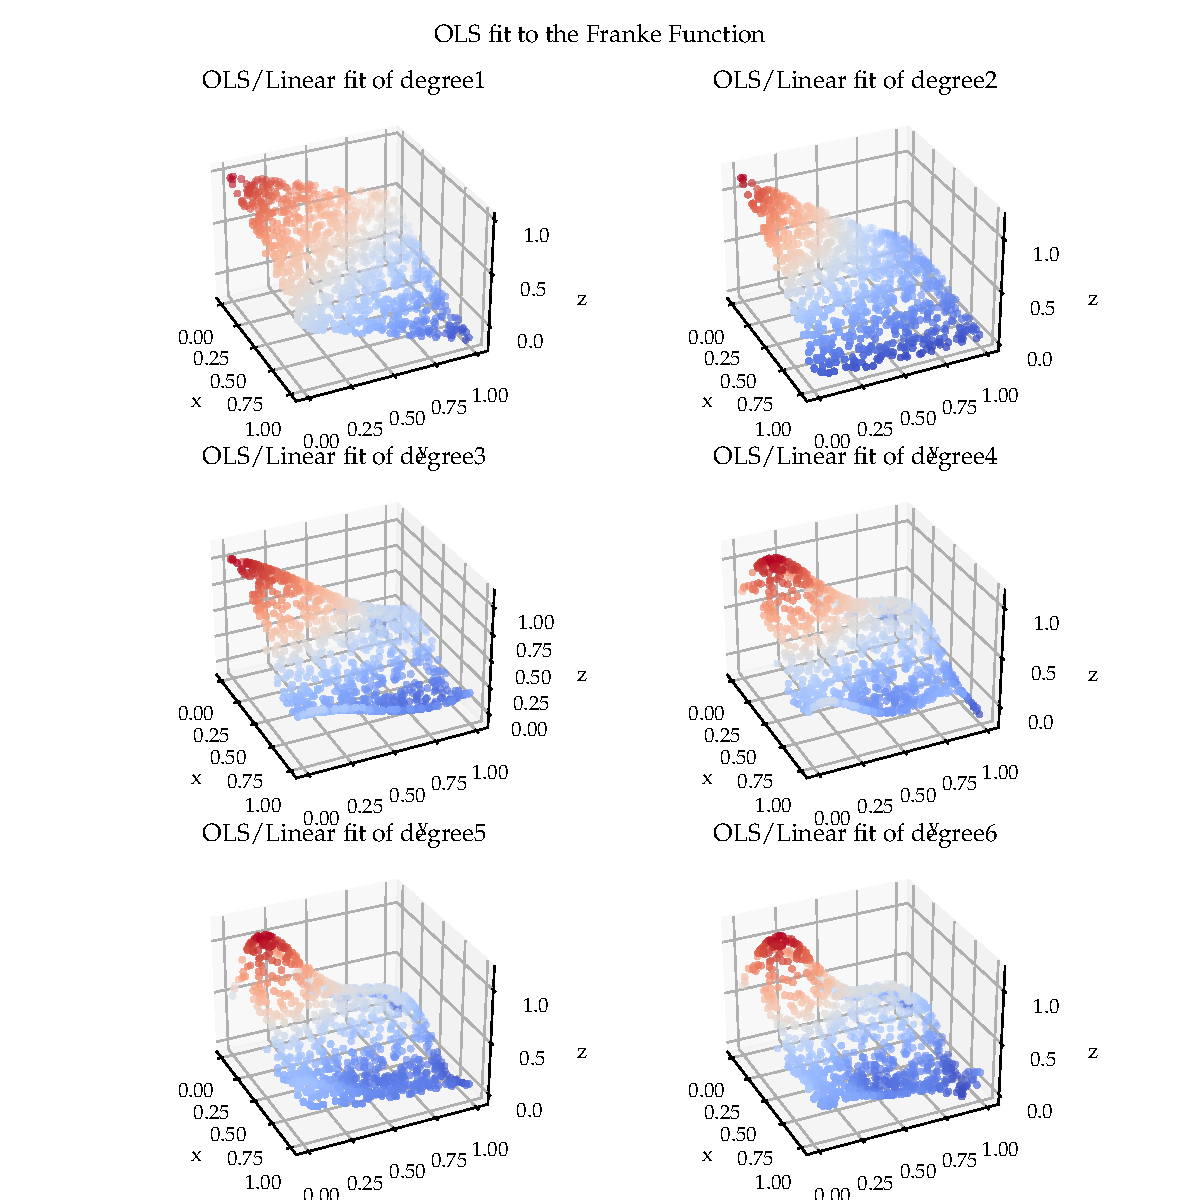
\includegraphics[scale=0.85]{figures/franke_function_OLS_fit.pdf}
  \caption{?}
  \label{fig: ?}
\end{figure}

\begin{figure}
  \centering
  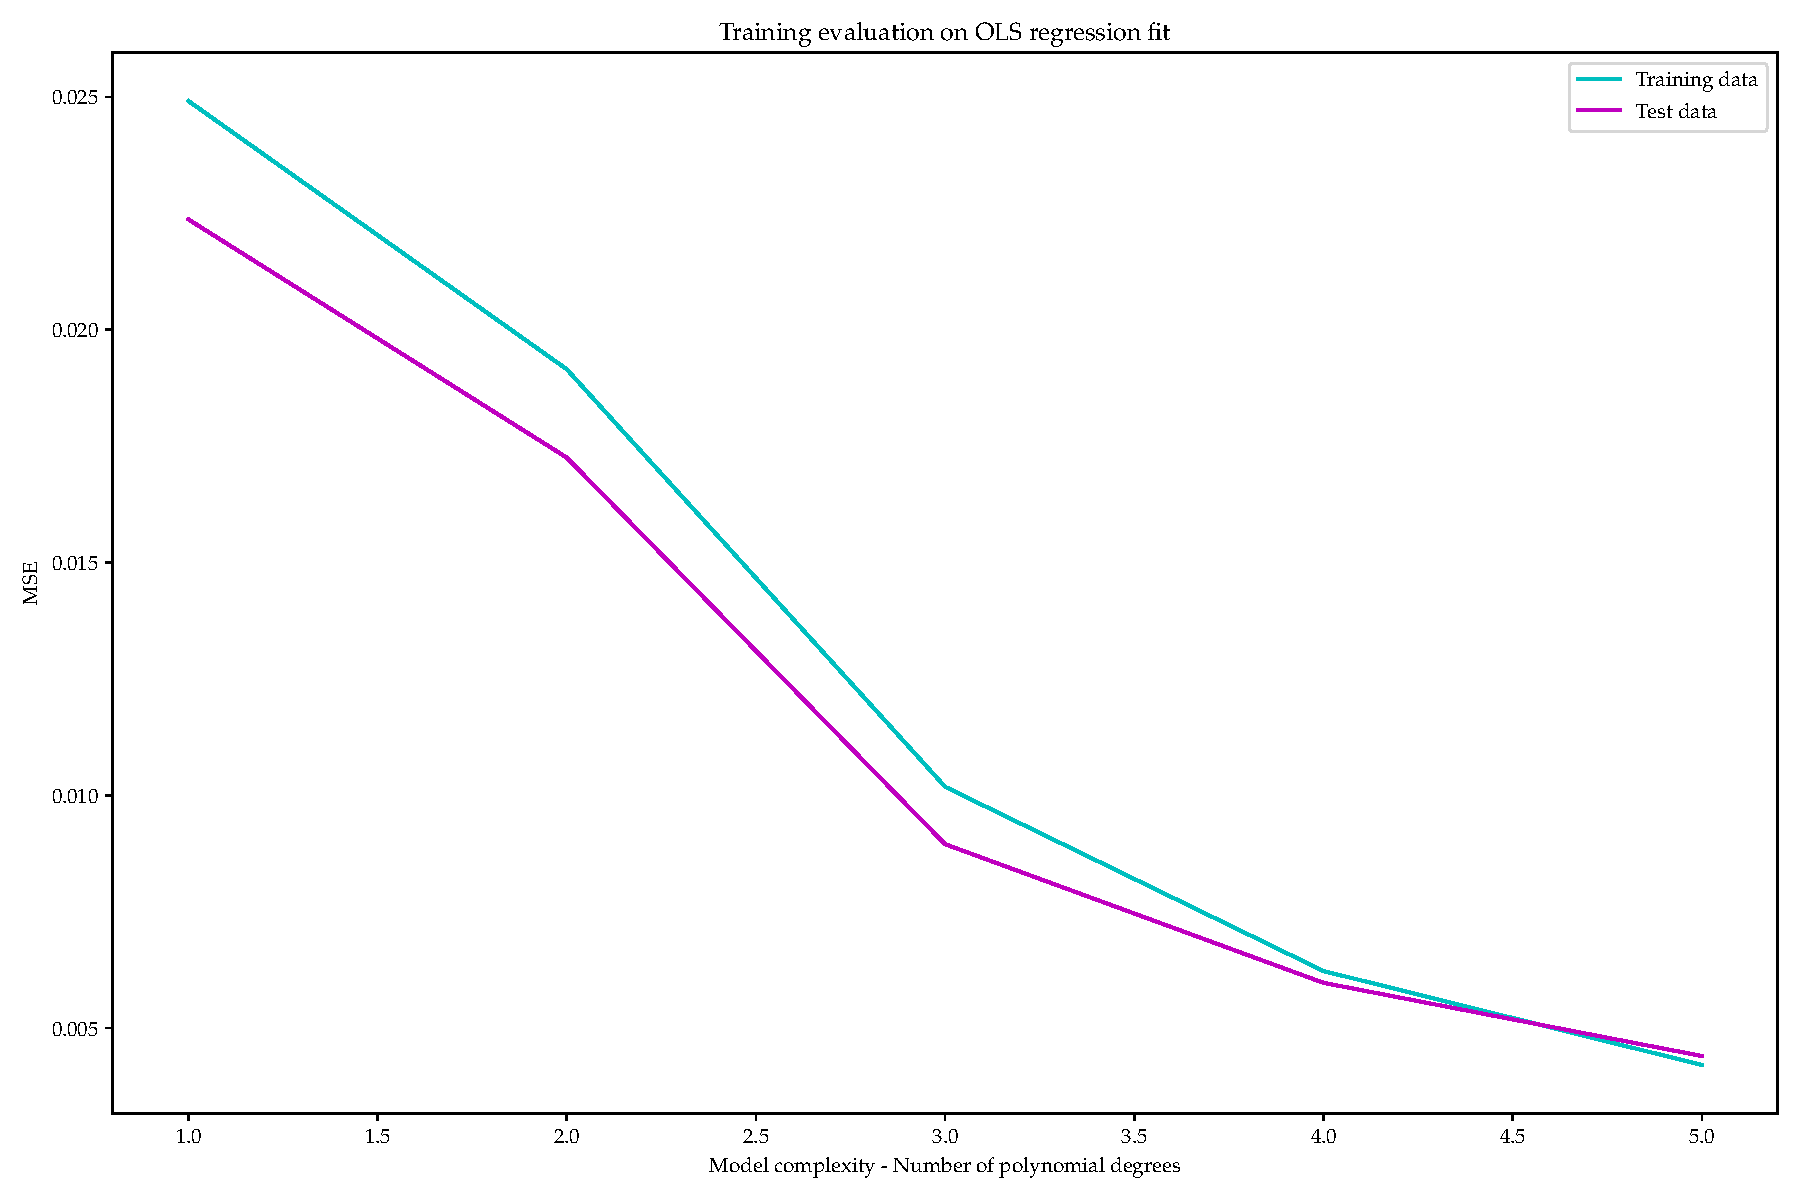
\includegraphics[scale=0.45]{figures/franke_function_OLS_evaluate_fit.pdf}
  \caption{?}
  \label{fig: ?}
\end{figure}

\begin{figure}
  \centering
  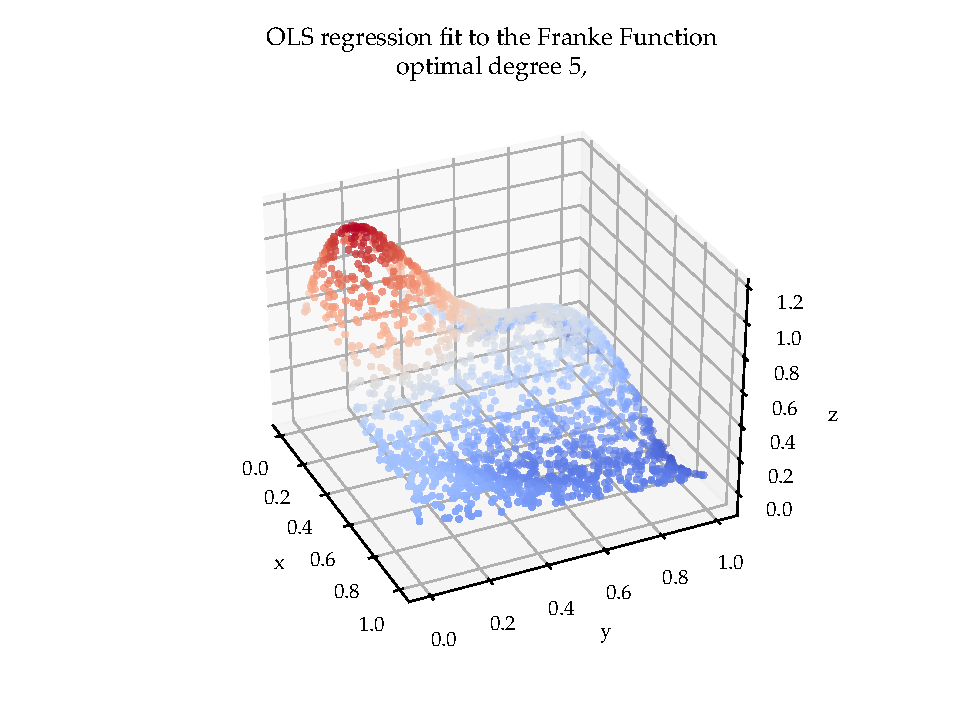
\includegraphics[scale=0.85]{figures/franke_function_OLS_best_fit.pdf}
  \caption{?}
  \label{fig: ?}
\end{figure}


\section*{Exercise 2}

\begin{figure}
  \centering
  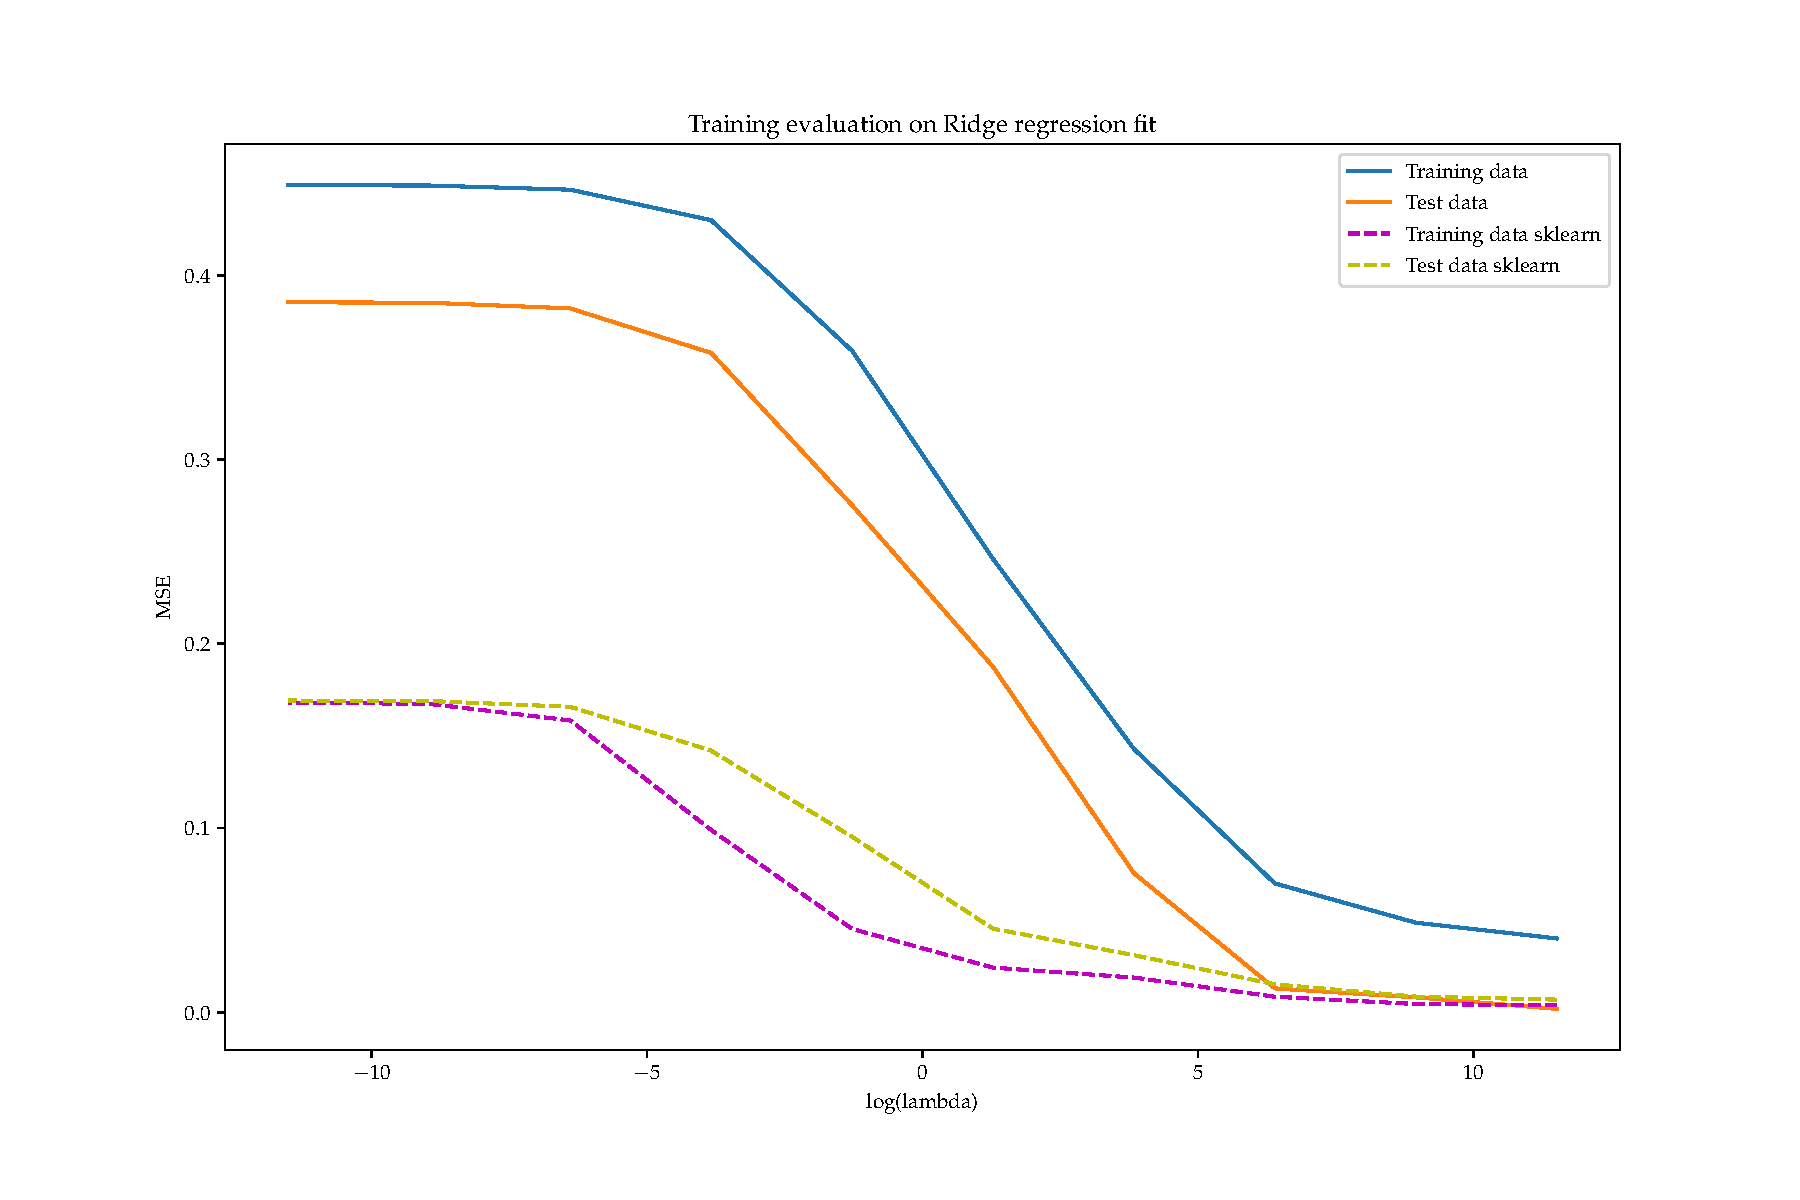
\includegraphics[scale=0.45]{figures/franke_function_Ridge_evaluate_fit.pdf}
  \caption{The best fit using Ridge}
  \label{fig: Ridge_best_fit}
\end{figure}

\begin{figure}
  \centering
  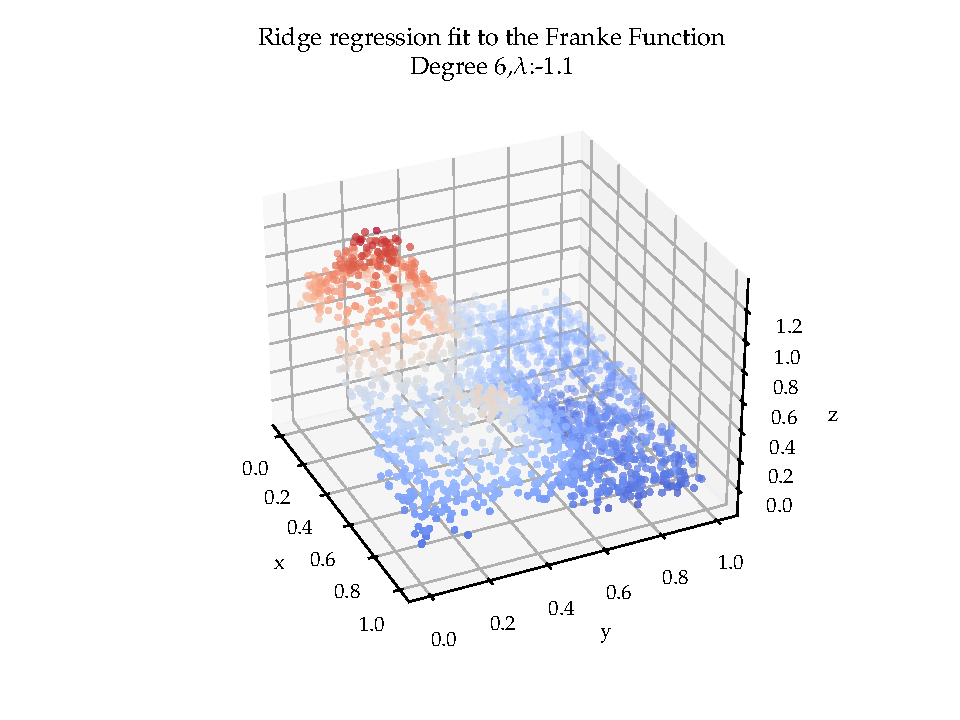
\includegraphics[scale=0.85]{figures/franke_function_Ridge_best_fit.pdf}
  \caption{The best fit using Ridge}
  \label{fig: Ridge_best_fit}
\end{figure}

\begin{center}
  \csvautobooktabular{data/report_data/redge_reg_lambda_-1.1.csv}
  \label{data: Ridge_best_fit}
\end{center}



\newpage
\newpage







\printbibliography


\end{document}


% Local Variables:
% TeX-engine: xetex
% End:
